\documentclass[12pt,a4paper]{report}
\usepackage[utf8]{inputenc}
\usepackage{graphicx}  % For including images
\usepackage{hyperref}
\usepackage{amsmath}
\usepackage{amssymb}
\usepackage{listings}
\usepackage{xcolor}
\usepackage{mdframed} % For colored boxes

\definecolor{codebg}{RGB}{240,240,240} % Background color for code listings
\definecolor{codecomment}{RGB}{150,150,150} % Comment color
\definecolor{codekeyword}{RGB}{0,0,255} % Keyword color
\definecolor{codestring}{RGB}{160,32,240} % String color

% Define code listing style
\lstdefinestyle{mystyle}{
    backgroundcolor=\color{codebg},   
    commentstyle=\color{codecomment},
    keywordstyle=\color{codekeyword},
    numberstyle=\tiny\color{codecomment},
    stringstyle=\color{codestring},
    basicstyle=\footnotesize\ttfamily,
    breakatwhitespace=false,         
    breaklines=true,                 
    captionpos=b,                    
    keepspaces=true,                 
    numbers=left,                    
    numbersep=5pt,                  
    showspaces=false,                
    showstringspaces=false,
    showtabs=false,                  
    tabsize=2
}

% Define colored box style for code listings
\mdfdefinestyle{mystyle}{
    backgroundcolor=codebg,
    roundcorner=5pt,
    innertopmargin=5pt,
    innerbottommargin=5pt,
    innerrightmargin=5pt,
    innerleftmargin=5pt,
    leftmargin=-10pt,
    rightmargin=-10pt,
}

% Apply the style to code listings
\lstset{style=mystyle}

\title{To-Do List Application}
\author{Aditi Dure}
\date{\today}

\begin{document}

\maketitle

\begin{abstract}
This report details the development of a to-do list application using Python. The application allows users to manage tasks by adding, viewing, completing, and deleting tasks. The report discusses the design, implementation, and usage of the application.
\end{abstract}

\tableofcontents

\chapter{Introduction}
\section{Purpose}
The purpose of this project is to create a simple and user-friendly to-do list application to help users manage their tasks efficiently.

\section{Scope}
The application provides functionalities to add new tasks, view the list of tasks, mark tasks as completed, and delete tasks. Completed tasks can also be viewed separately.

\chapter{Design and Implementation}
\section{Design Approach}
The application is designed with simplicity and ease of use in mind. It employs a command-line interface where users can interact with the to-do list through various options.

\section{Modules and Functions}
\subsection{Task Manager Module}
The main functionality is encapsulated in a module named \texttt{task\_manager.py}, which handles all task-related operations.

\subsubsection{Data Structures}
\begin{itemize}
    \item \texttt{tasks}: A list to store current tasks.
    \item \texttt{completed\_tasks}: A list to store completed tasks.
\end{itemize}

\subsubsection{Functions}
\begin{itemize}
    \item \texttt{load\_tasks\_from\_file(filename)}: Loads tasks from a specified file.
    \item \texttt{load\_completed\_tasks\_from\_file(filename)}: Loads completed tasks from a specified file.
    \item \texttt{save\_tasks\_to\_file(filename)}: Saves current tasks to a specified file.
    \item \texttt{save\_completed\_tasks\_to\_file(filename)}: Saves completed tasks to a specified file.
    \item \texttt{add\_task(task)}: Adds a new task to the list.
    \item \texttt{view\_tasks()}: Displays all current tasks.
    \item \texttt{complete\_task(task\_index)}: Marks a task as completed.
    \item \texttt{delete\_task(task\_index)}: Deletes a task from the list.
    \item \texttt{view\_completed\_tasks()}: Displays all completed tasks.
\end{itemize}

\section{Data Storage}
The tasks and completed tasks are stored in separate text files:
\begin{itemize}
    \item \texttt{to\_do\_list.txt}: This file stores the current tasks.
    \item \texttt{completed\_tasks.txt}: This file stores the completed tasks.
\end{itemize}

\section{Main Program}
The main program provides a command-line interface for interacting with the to-do list. It handles user input and calls the appropriate functions from the \texttt{task\_manager} module.

\chapter{Usage}
\section{Running the Application}
To run the application, execute the main program script. The user will be presented with a menu of options to interact with the to-do list.

\section{Features}
\begin{itemize}
    \item \textbf{Add Task}: Allows the user to add a new task to the list.
    \item \textbf{View Tasks}: Displays all current tasks.
    \item \textbf{Mark Task as Completed}: Marks a specified task as completed.
    \item \textbf{Delete Task}: Deletes a specified task from the list.
    \item \textbf{View Completed Tasks}: Displays all tasks that have been marked as completed.
    \item \textbf{Exit}: Exits the application.
\end{itemize}

\section{Result Screenshots}
\begin{figure}[htbp]
    \centering
    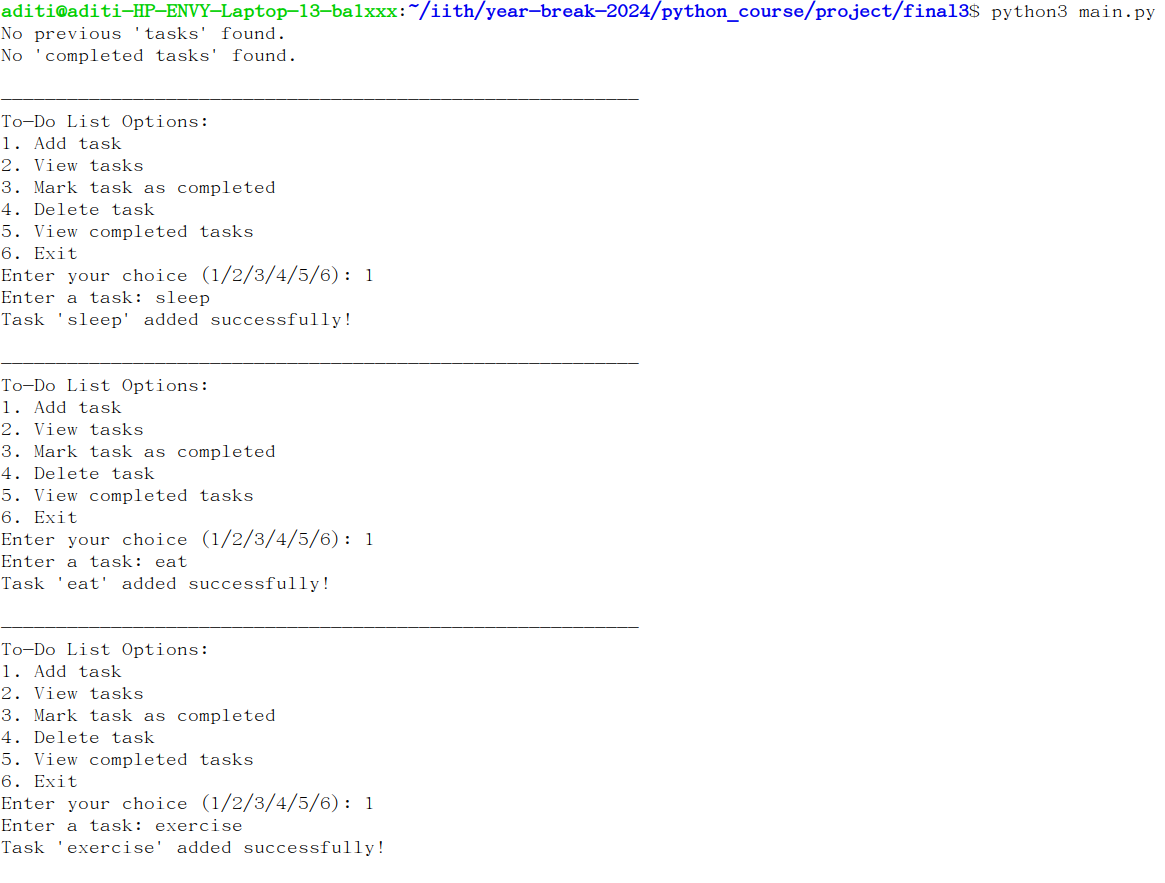
\includegraphics[width=1\textwidth]{./figs/1.png}
    \caption{terminal}
    \label{fig:ss1}
\end{figure}

\begin{figure}[htbp]
    \centering
    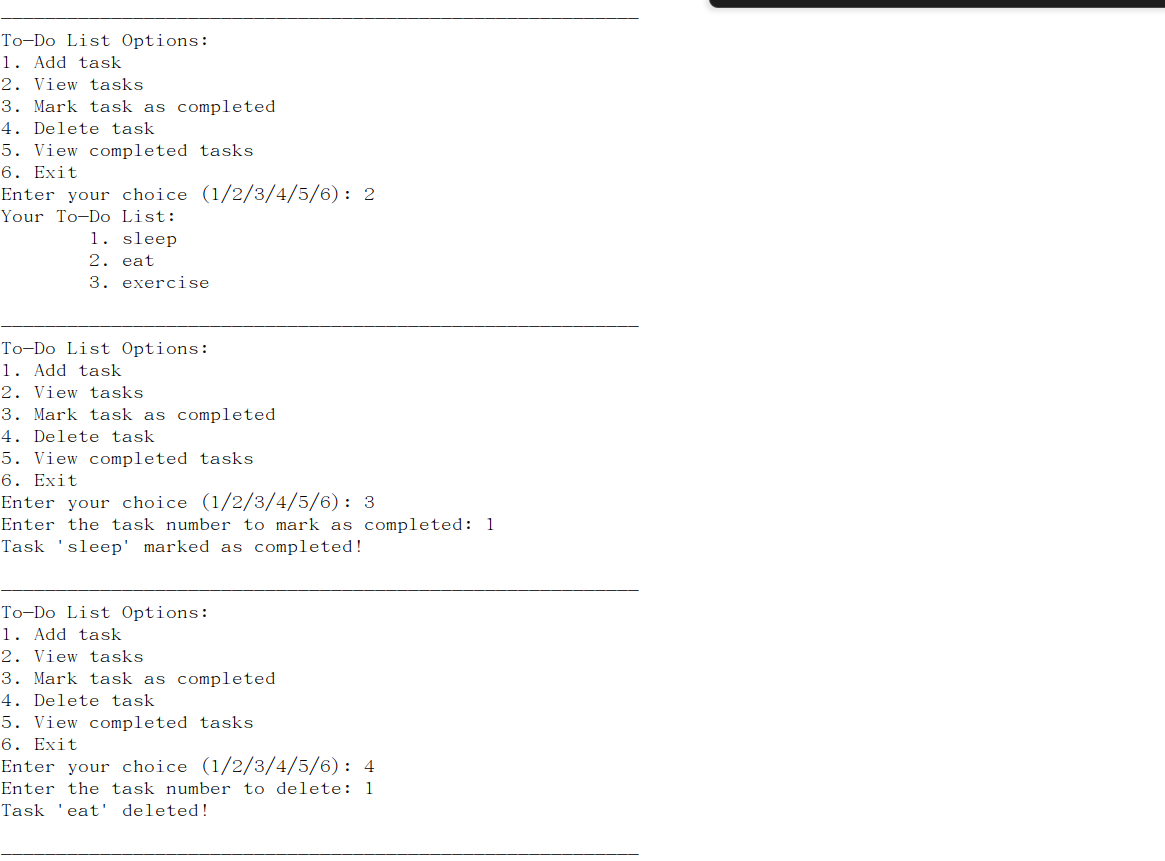
\includegraphics[width=1\textwidth]{./figs/2.png}
    \caption{terminal}
    \label{fig:ss2}
\end{figure}

\begin{figure}[htbp]
    \centering
    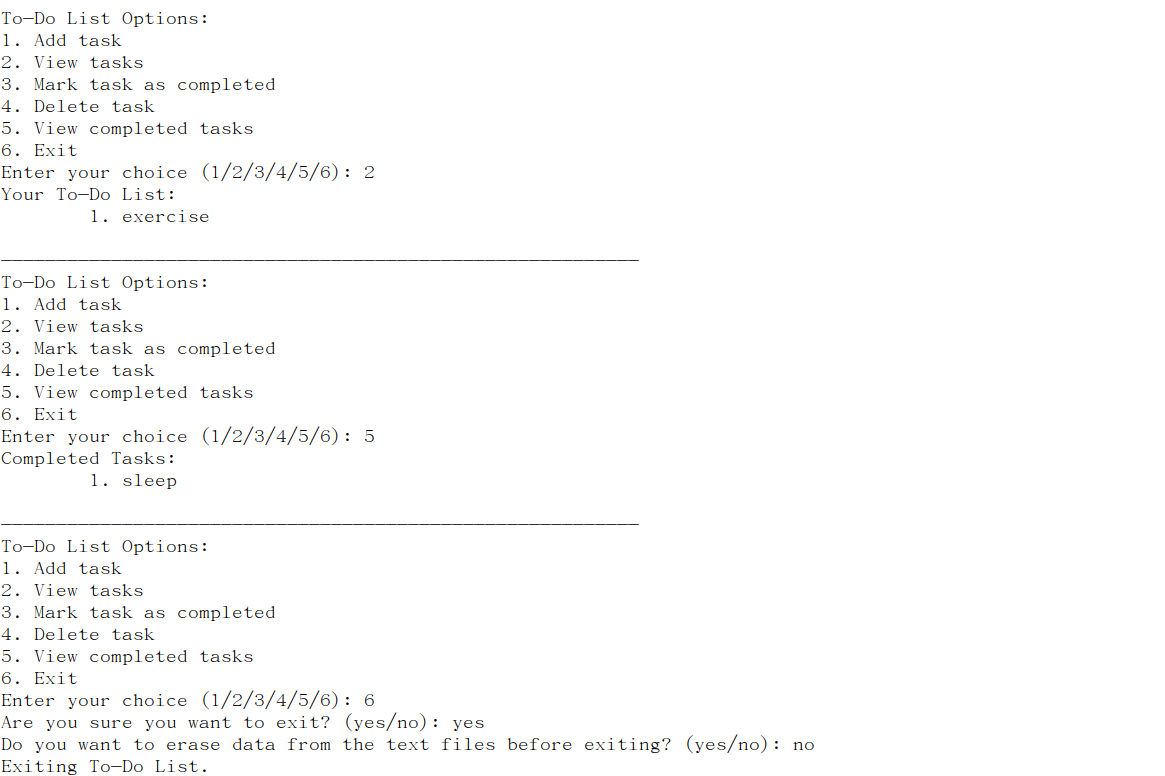
\includegraphics[width=1\textwidth]{./figs/3.png}
    \caption{terminal}
    \label{fig:ss3}
\end{figure}

\begin{figure}[htbp]
    \centering
    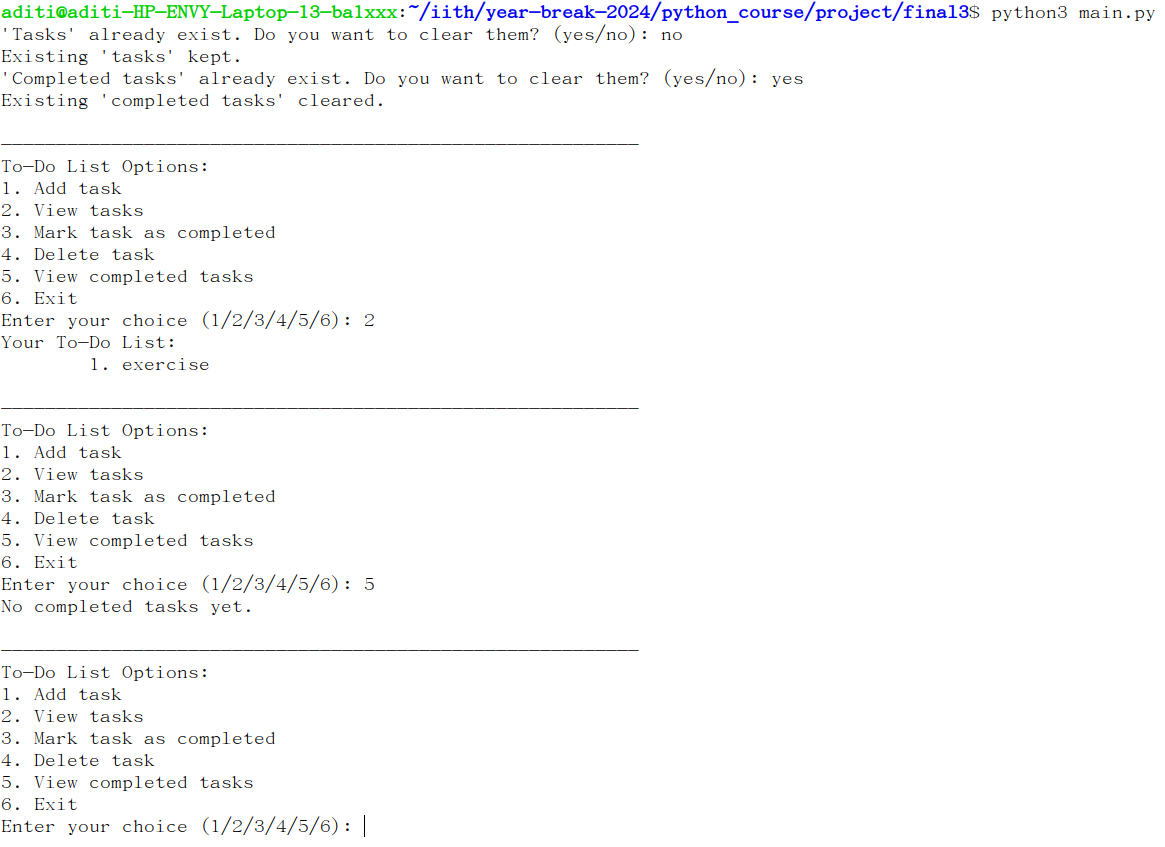
\includegraphics[width=1\textwidth]{./figs/4.png}
    \caption{terminal}
    \label{fig:ss4}
\end{figure}

\begin{figure}[htbp]
    \centering
    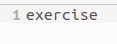
\includegraphics[width=0.2\textwidth]{./figs/a.png}
    \caption{to\_do\_list.txt}
    \label{fig:ssf1}
\end{figure}

\begin{figure}[htbp]
    \centering
    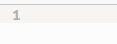
\includegraphics[width=0.2\textwidth]{./figs/b.png}
    \caption{completed\_tasks.txt}
    \label{fig:ssf2}
\end{figure}

\chapter{Conclusion}
The to-do list application provides a simple and effective way for users to manage their tasks. Future improvements could include a graphical user interface and additional features such as task prioritization and reminders.

\appendix
\chapter{Code Listings}
\section{\texttt{task\_manager.py}}
\begin{mdframed}[style=mystyle]
\lstinputlisting[language=Python, caption=Task Manager Module]{./codes/task_manager.py}
\end{mdframed}

\section{\texttt{main.py}}
\begin{mdframed}[style=mystyle]
\lstinputlisting[language=Python, caption=Main Program]{./codes/main.py}
\end{mdframed}

\chapter{References}
\begin{itemize}
    \item Python Course: Techgyan.
\end{itemize}

\end{document}


